% !TEX TS-program = pdflatexmk
\documentclass{styles/assisi}
\DeclareRobustCommand{\DelivNumber}{Circular setup configuration}
\DeclareRobustCommand{\DelivName}{\today}
\DeclareRobustCommand{\DelivStatus}{Confidential}
\DeclareRobustCommand{\DelivRevision}{0.1}
\DeclareRobustCommand{\DeliveryDate}{}
\DeclareRobustCommand{\DelivPartnersOwning}{\bf EPFL}
\DeclareRobustCommand{\DelivPartnersContributing}{\bf PARIS7}
\DeclareRobustCommand{\DelivPartnersContributingNextLine}{}
\DeclareRobustCommand{\DelivDue}{N/A}
\DeclareRobustCommand{\DelivAbstract}{This tutorial explains how to generate the circular setup configuration file for CATS2.}

%----------------------------------------------------------------------------------------------
\makeindex

\usepackage{epsfig,subfigure,float,pseudocode,multirow,footmisc,rotating}
\usepackage{graphicx}        % standard LaTeX graphics tool
\usepackage{amsmath, amssymb, subfigure}
\usepackage{multirow, rotating}
\usepackage[ruled,lined,commentsnumbered]{algorithm2e}
\usepackage[colorlinks=false, urlcolor=blue, pdfborder={0 0 0}]{hyperref}
%\usepackage{algorithm2e}
\usepackage{pdfpages}
\usepackage{afterpage}
\usepackage{booktabs}
\usepackage{geometry}
\usepackage{listings}
\usepackage{color}

\newcommand{\rd}{\Delta^{\frac{1}{2}}}
\newcommand{\pla}{\phi_{\lambda_1}^t}
\newcommand{\plb}{\phi_{\lambda_2}^t}
\newcommand{\ie}{i.\,e.,\ }
\newcommand{\Ie}{I.\,e.,\ }
\newcommand{\eg}{e.\,g.,\ }
\newcommand{\Eg}{E.\,g.,\ }
\newcommand{\assisi}{ASSISI$|_{bf}$ }
\setcounter{tocdepth}{3}

% TODO command
\newcommand{\todo}[1]{\par\noindent{\raggedright\textsc{\color{red}#1}%
    \par\marginpar{{\Large\color{red}$\star$}}}}

\begin{document}
\thispagestyle{plain}
  \vspace*{0.3cm}
  \begin{center}
  {\bf \LARGE SEVENTH FRAMEWORK PROGRAMME}\\
  \vspace*{0.6cm}
  
\includegraphics[width=0.15\textwidth]{styles/7th.png}\\
  \vspace*{2.0cm}
  \bf {\large IP}\\
  \vspace*{1.0cm}
  \bf {\Huge ASSISIbf}\\
  \vspace*{.6cm}
  \bf {\it \Large Animal‌ and‌ robot‌ Societies‌ ‌Self-organise‌ and‌ Integrate‌ by‌ Social‌ Interaction‌ (bees‌ and‌ fish)‌}\\
  \vspace*{45pt}
  {\huge \bf \DelivNumber}\\
  \vspace*{12pt}
  {\Large \it \bf \DelivName}\\
  \vspace*{70pt}
  \small
  \begin{tabular}{|ll|}
    \hline &\\
    Date of preparation: \DeliveryDate & Revision: \DelivRevision\\ &\\
    Start date of project: February 1st, 2013 & Duration: 60 months\\ &\\
    Project co-ordinator: UNIGRAZ & Classification: \DelivStatus \\ &\\
    Partners: & \\
    %& \\
    ~~{\it owning:} \DelivPartnersOwning &~~{\it contributed:} \DelivPartnersContributing\\
    &\DelivPartnersContributingNextLine\\
    &\\
    Project website: & http://assisi-project.eu\\
    &\\
    \hline
  \end{tabular}
  \end{center}
%\newpage
%
%%-----------------------------------------------------------------
%\begin{center}
%\begin{tabular}{|lp{10cm}|}
%\hline &\\
%\multicolumn{2}{|c|}{\bf \Large DELIVERABLE SUMMARY SHEET} \\
%&\\
%\hline \hline
%&\\
%Project Number: & 601074\\
%&\\
%Project Acronym: & {\bf ASSISIbf}\\
%&\\
%Title:     & Animal‌ and‌ robot‌ Societies‌ ‌Self-organise‌ and‌ Integrate‌ by‌ Social‌ Interaction‌ (bees‌ and‌ fish) \\
%&\\
%\hline \hline
%&\\
%Deliverable N$^o$: & \DelivNumber\\
%&\\
%Due Date: & Project month: \DelivDue\\
%&\\
%Delivery Date: & \DeliveryDate \\
%&\\
%\hline \hline
%&\\
%\textbf{Name:} & {\bf \DelivName}\\
%&\\
%\textbf{Description:} & \DelivAbstract\\
%&\\
%&\\
%\hline \hline
%&\\
%Partners owning: & \DelivPartnersOwning \\
%&\\
%&\\
%Partners contributed: & \DelivPartnersContributing ~\DelivPartnersContributingNextLine \\
%&\\
%&\\
%Made available to: & \DelivStatus\\
%&\\
%\hline
%\end{tabular}
%\end{center}
%%}{}



%------------------------------------------------------------------



\textsf{\tableofcontents}
%\textsf{\listoffigures}
%\addcontentsline{toc}{chapter}{List of Figures}
%\textsf{\listoftables} \addcontentsline{toc}{chapter}{List
%of Tables}

\lstset{
    language=xml,
    tabsize=3,
    %frame=lines,
    %caption=Test,
    %label=code:sample,
    %frame=shadowbox,
    %rulesepcolor=\color{gray},
    xleftmargin=20pt,
    framexleftmargin=15pt,
    %keywordstyle=\color{blue}\bf,
    %commentstyle=\color{OliveGreen},
    %stringstyle=\color{red},
    numbers=left,
    numberstyle=\tiny,
    numbersep=5pt,
    breaklines=true,
    showstringspaces=false,
    basicstyle=\footnotesize}

\chapter{Introduction}\label{chap:intro}
In this tutorial we will show how to generate the setup file for the circular arena as well the control areas (or zones). As as example, we will use the {\it cats2-epfl-binary-choice.xml} configuration file that can be found in the {\it config} folder in CATS2.

\chapter{Model configuration}\label{chap:intro}
\section{Install the setup}
Carefully install the experimental setup, it should not be moved later. 

\section{Generate polygons from the arena view}
Take the setup print screen from CATS2. Open it in any image editor that allows to get the pixels positions under the cursor (position $(0,0)$ in the left-top corner). 

Open the {\it circular-setup-map-generator.py} file from the {\it scripts/circular-setup} folder and adjust {\it internalRadiusPx}, {\it externalRadiusPx}, {\it xCenterPx} and {\it yCenterPx} parameters based on the position and the size of the setup circle on the setup. 

Run the script, it will generate files {\it innerCircle.txt} and {\it outerCircle.txt} in the {\it results} folder. Now these files need to be converted to the world coordinates. To do this use {\it cooridinates-convertor} application from the CATS2 examples. It takes the following parameters: 
\begin{itemize}
\item {\it -c  <path-to-the-configuration-file>}: the configuration file stores the path to the camera calibration file;
\item {\it -wh 1/0}: defines if the first line in the file is the header and needs to be skipped;
\item {\it -st mainCamera/cameraBelow}: is the setup type for the view used to get the dimensions of the circular setup;
\item {\it -i <input-text-file-to-convert>}: the path to the input file
\end{itemize}

Pass each of two text files to {\it cooridinates-convertor}, it will generate {\it xml} files with the corresponding world positions.

\section{Define the setup map file}
The {\it xml} file with the setup map is to be copied to the {\it config/setup} folder. In the CATS2 configuration file the setup map is defined under {\it experiment/setupMapPath}. Once set it will be automatically shown in CATS2. As an example of the setup map have a look on the {\it epfl-circular.xml}. It's recommended to place the print screen with the setup to  {\it config/setup} folder, with the same name as the setup map file, e.g. {\it epfl-circular.png}

Make a new setup file in {\it config/setup} folder. Copy the polygon from {\it outerCircleWorld.xml} file to the {\it polygon} section of the setup file, and the polygon from the {\it innerCircleWorld.xml} file to the {\it excluded polygons} section.  

\begin{figure}[ht]
\centering
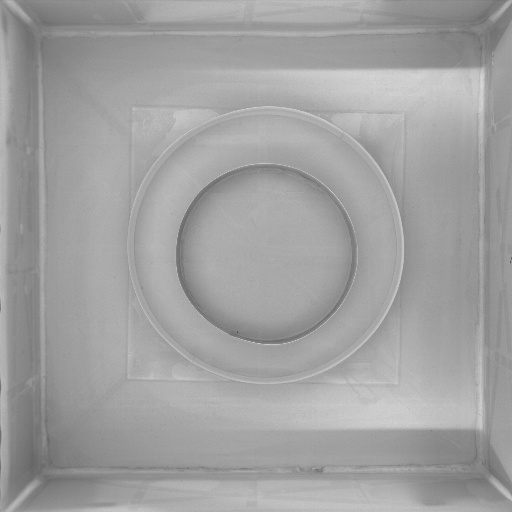
\includegraphics[width=0.4\textwidth]{./figs/epfl-circular.png}
\caption{The main view of CATS2 with the setup map shown above the fish two-rooms setup.}
\label{fig:setup-map}
\end{figure}

\section{Define the zones in the control map}
The python script also generates the sector areas, you can specify their number by changing the {\it sectorsNumber} parameter, they have names {\it room-1}, {\it room-2}, etc. You can convert them to the world coordinates and to use to define the control areas or zones for the model. 

\subsection{Create the control map}
The control map files are stored in the {\it config/control-maps} folder. For the reference check {\it epfl-four-sectors-control-map.xml}. 

Once the control map file is done, it should be set in the configuration file at {\it robots/controllers/controlMap/controlAreasPath} and then to see the zones in CATS2 one can simply activate the {\it Control map} experiment. 

\begin{figure}[ht]
\centering
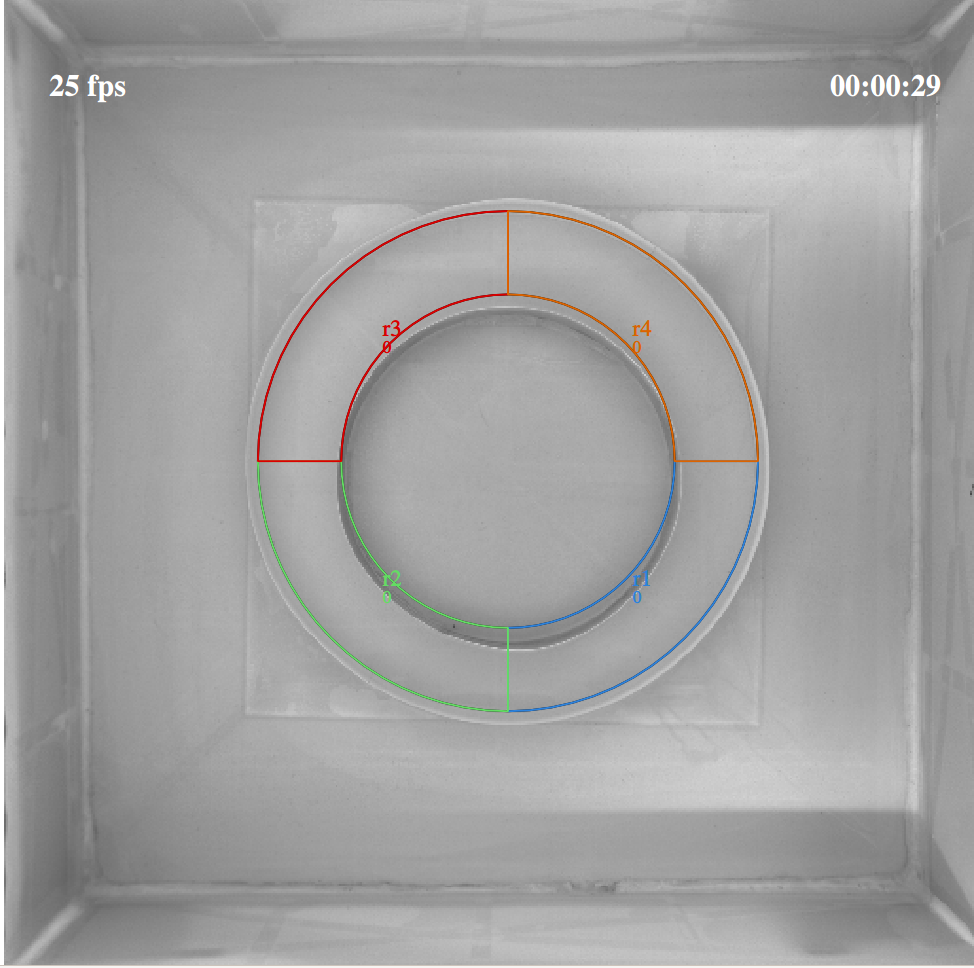
\includegraphics[width=0.4\textwidth]{./figs/epfl-circular-zones.png}
\caption{The main view of CATS2 with the control areas.}
\label{fig:control-areas}
\end{figure}

\end{document}

